%Copyright  Jean-Philippe Eisenbarth
%This program is free software: you can 
%redistribute it and/or modify it under the terms of the GNU General Public 
%License as published by the Free Software Foundation, either version 3 of the 
%License, or (at your option) any later version.
%This program is distributed in the hope that it will be useful,but WITHOUT ANY 
%WARRANTY; without even the implied warranty of MERCHANTABILITY or FITNESS FOR A 
%PARTICULAR PURPOSE. See the GNU General Public License for more details.
%You should have received a copy of the GNU General Public License along with 
%this program.  If not, see <http://www.gnu.org/licenses/>.

%Based on the code of Yiannis Lazarides
%http://tex.stackexchange.com/questions/42602/software-requirements-specification-with-latex
%http://tex.stackexchange.com/users/963/yiannis-lazarides
%Also based on the template of Karl E. Wiegers
%http://www.se.rit.edu/~emad/teaching/slides/srs_template_sep14.pdf
%http://karlwiegers.com
\documentclass{scrreprt}
\usepackage{array}
\usepackage{listings}
\usepackage{underscore}
\usepackage[bookmarks=true]{hyperref}
\usepackage[utf8]{inputenc} 
\usepackage[english]{babel}
\usepackage{textcomp}
\usepackage{graphicx} %utilisation d'images
\usepackage{enumitem}
\usepackage[T1]{fontenc}
\usepackage{times}
\hypersetup{
    bookmarks=false,    % show bookmarks bar?
    pdftitle={Software Requirement Specification},    % title
    pdfauthor={Jean-Philippe Eisenbarth},                     % author
    pdfsubject={TeX and LaTeX},                        % subject of the document
    pdfkeywords={TeX, LaTeX, graphics, images}, % list of keywords
    colorlinks=true,       % false: boxed links; true: colored links
    linkcolor=blue,       % color of internal links
    citecolor=black,       % color of links to bibliography
    filecolor=black,        % color of file links
    urlcolor=purple,        % color of external links
    linktoc=page            % only page is linked
}%
\def\myversion{1.0 }
\date{}
%\title
\usepackage{hyperref}
\begin{document}

\begin{flushright}
    \rule{15cm}{5pt}\vskip1cm
    \begin{bfseries}
        \Huge{SOFTWARE REQUIREMENTS\\ SPECIFICATION}\\
        \vspace{1.0cm}
        for\\
        \vspace{1.0cm}
        Gestionnaire de Stage Telecom Nancy\\
        \vspace{1.0cm}
        \LARGE{version \myversion approved}\\
        
        \vspace{1.0cm}
        Prepared by \\ 
        \vspace{1.0cm}
        \begin{flushleft}
        Alexandre CHICHMANIAN \\ Gauthier ZAMBAUX \\ Mouchid WAIDI \\ Guillaume GARCIA\\
        \end{flushleft}
        \vspace{1.0cm}
        Los Pollos\\
        \vspace{1.0cm}
        \today\\
    \end{bfseries}
\end{flushright}

\renewcommand{\contentsname}{Contenu}
\tableofcontents


%\chapter*{Revision History}

%\begin{center}
   % \begin{tabular}{|c|c|c|c|}
      %  \hline
	 %   Name & Date & Reason For Changes & Version\\
        %\hline
	   % 21 & 22 & 23 & 24\\
        %\hline
	   % 31 & 32 & 33 & 34\\
        %\hline
   % \end{tabular}
%\end{center}

\chapter{INTRODUCTION}

\section{A propos de ce document}
\hspace{1cm}Ce document a pour objectif de présenter l'application de gestion des stages de Télécom Nancy, d'en donner les acteurs et les fonctionnalités ainsi que les contraintes qui y sont associées. Il présente par ailleurs aussi l'interface graphique de l'application.

\section{Portée du document}
\hspace{1cm}L'application présentée ici a pour objectif de facilité la gestion des stages des étudiants de Télécom Nancy.\\

\hspace{0.6cm}Du point de vue administratif, elle facilite la gestion des stages en permettant la création de bases de données évitant la recopie manuelle d'informations. Les conventions de stage sont notamment générée automatiquement.\\

\hspace{0.6cm}Par le biais de cette application, les étudiants ont la possibilité de saisir directement les informations relatives à leur stage, d'obtenir les informations dont ils peuvent avoir besoin (par exemple avec le livret de l'élève) et de rendre leur rapport de stage en ligne.\\

\hspace{0.6cm}Finalement, l'application permet aux professeurs référents de communiquer avec les étudiants, de récupérer les rapports à corriger et de valider ou non les stages de élèves.

\section{Public concerné et vue d'ensemble du document }

\hspace{1cm}Ce cahier des charges visent avant tout les instigateurs et responsables du projet ainsi que les développeurs. Par extension, il peut aussi être utile pour les futurs utilisateurs de l'application, c'est-à-dire les étudiants, les professeurs et l'administration de Télécom Nancy.\\

\hspace{0.6cm}La première partie de ce document introduit les objectifs principaux de l'applications ainsi que les personnes visées. Elle se charge aussi de définir les conventions de rédaction du cahier de charge.\\

\hspace{0.6cm}La deuxième partie se concentre sur une description plus détaillée des fonctionnalités attendues et de l'environnement d'évolution de l'application, notamment son adaptabilité aux utilisateurs.\\

\hspace{0.6cm}La troisième partie présente l'interface utilisateur ainsi que les différentes contraintes auxquelles le logiciel doit se plier.\\

\hspace{0.6cm}La quatrième partie présente les besoins non fonctionnels non présentés précédemment.\\

\hspace{0.6cm}Finalement, les annexes présentent le dictionnaire des données et le diagramme entités-associations.

\section{Définitions, acronymes et abréviations}
\hspace{1cm}Voici une liste des différentes abréviations utilisées dans ce document :
\begin{description}
\item[CAS :] Central Authentification Service service d'authentification de l'UL
\item[UL :] Université de Lorraine
\item[SMTP :] Simple Mail Transfer Protocol , protocole qui permet de recevoir des messages électroniques d'une boite mail existante( idpersonne@telecomnancy.eu)
\item[IMAP :] Internet Message Access Protocol, protocole qui permet d'envoyer un message électronique sans passer par sa boite mail directement.
%\item[HTTPS :]​ Hypertext Transfer Protocol Secure, protocole sécurisé qui permet l'échange entre client et serveur


\end{description}

\section{Conventions de rédaction du document}

\hspace{1cm}L'intégralité de ce document a été écrit avec la police Times New Roman.\\

\hspace{0.6cm}Lorsqu'une personne est citée, son nom est écrit en majuscule, et son prénom, seule la première lettre est en majuscule.

\section{Références et remerciements}
\hspace{1cm}Afin de pouvoir réaliser nos schémas, nous avons utilisé le logiciel : 

\hspace{1cm}- balsamiq (création des interfaces étudiant/secrétaire) \\

\hspace{0.6cm}et les sites internet :

\hspace{1cm}- plantuml.com (diagram pattern)

\hspace{1cm}- l'application de Mouchid (Diagrammes UML)\\

\hspace{0.6cm}Notre site internet fait réference :

\hspace{1cm}- au CAS de l'Université de Lorraine pour la connection unique et sécurisé de chacun

\hspace{1cm}- à la boite mail de Telecom Nancy (https://webmail.telecomnancy.eu) pour pouvoir échanger directement depuis le site internet.\\
	

\chapter{DESCRIPTION GLOBALE }

\section{Perspective du produit}

\hspace{1cm}Le site web Gestionnaire de Stages Telecom Nancy a pour but de faciliter le suivi des stages des étudiants de Telecom Nancy.\\

\hspace{0.6cm}Elle permet dans un premier temps de créer de façon automatique, la fiche de renseignements du stage, et la convention de stage. Pour cela, le site web sera optimisé aussi bien pour ordinateur que pour smartphone ou tablette et permettra des échanges entre les élèves, la secrétaire des stages et les professeurs. L'école, étant rattaché désormais à l'Université de Lorraine, la connection sur la plate-forme se fera grâce au système d'authentification CAS.

\section{Fonctionnalités du produit}
L'application web va permettre aux étudiants de :
\begin{itemize}[label=\textbullet]
	\item Créer automatique des fiches de renseignement des stages en fonction des donnée entrées par l'étudiant
	\item Créer automatique de la convention de stage
	\item Communiquer entre élèves et professeurs
	\item Récupérer le livret de stages
	\item Récupérer la fiche d'évaluation
	\item Récupérer des templates mémoire ingénieur
	\item Envoyer sur le serveur la fiche d'évaluation remplie
	\item Envoyer le rapport de stage/mémoire ingénieur sur le serveur
	\item Consultater des offres de stages disponibles
	\item Consultater de la date de soutenance son horaire et sa salle
\end{itemize}

L'application web va permettre à la secrétaire des stages de :
\begin{itemize}[label=\textbullet]
	\item Déposer le livret des stages sur la plateforme
	\item Déposer la fiche d'évaluation vierge
	\item Récupérer les fiches récapitulatif de stage
	\item Récupérer les conventions de stages signées
	\item Récupérer les rapports de stage/mémoire ingénieur
	\item Mettre en ligne les offres de stages
	\item Entrer les dates de soutenance avec l'horaire et la salle
	\item Modifier le statut des élèves ( 1A / 2A / 3A)
	
\end{itemize}
	

\section{Utilisateurs}
\hspace{1cm}Ce site internet sera avant tout utilisé par les étudiants afin de pouvoir préparer leur stage du début de leurs recherche jusqu'à la date de la soutenance. Il sera aussi utilisé par la secrétaire des stages qui sera là pour mener à bien la préparation des stages des étudiants. Il sera aussi utilisé par les professeurs afin de connaitre les soutenances auxquelles ils devront prendre part, mais ce site sera aussi utilisé par les référents de stages afin de mener à bien la préparation des élèves, et de communiquer avec eux si nécessaire.\\

\hspace{0.6cm}Dans tous les cas, tout utilisateur va devoir se connecter sur la plateforme grâce au CAS de l'université de Lorraine.

\section{Environnement d'exécution}
\hspace{1cm}L'application développée ici est une application web et doit de ce fait pouvoir fonctionner avec les navigateurs internet les plus courants (Edge, Firefox, Chrome en particulier).\\

\hspace{0.6cm}De plus, les utilisateurs doivent pouvoir y avoir accès sur différentes plateformes, notamment les ordinateurs, les smartphones et les tablettes. Elle doit aussi être supportée par les systèmes d'exploitation les plus courants (Windows, les distributions Linux, OSX, Android, iOS et Windows Phone).\\

\hspace{0.6cm}L'application permet l'authentification de ses utilisateurs par le biais du CAS de l'UL, et dispose de sa propre base de données des informations sur les élèves. Elle est hébergée par les serveurs de l'UL et doit avoir accès à suffisemment d'espace mémoire pour stocker les documents tels que le livret de l'élève et les rapports de stage des étudiants lorsque ceux-ci les y déposent.


\section{Contraintes de conception et d'implémentation}
\hspace{1cm}L'application web que nous developpons ici doit être écrite en langages HTML/CSS et PHP ou Javascript. Le langage MySQL sera utilisé pour les bases de données nécessaires au bon fonctionnement de l'application.\\

\hspace{0.6cm}Elle doit pouvoir fonctionner sur différents types de supports et systèmes d'exploitation, et doit notamment s'adapter à la taille de l'écran que l'utilisateur utilise. Elle doit aussi être légère puisque les smartphone ne permettent pas l'utilisation d'application trop demandeuses de ressources.\\

\hspace{0.6cm}L'application doit pouvoir être utilisable et maintenable par le service information de Télécom Nancy sans que cela n'empiète sur leur travail.


\section{Manuel utilisateur}
\hspace{1cm}Un manuel utilisateur est prévu pour que les étudiants et les membres du service scolarité puissent apprendre à utiliser l'application. Il sera par ailleurs possible de contacter le service informatique depuis le site internet pour assistance.


\section{Hypothèses et dépendances}
\hspace{1cm}L'application suppose que les personnes amenées à l'utiliser possèdent toutes des identifiants leur permettant de se connecter au CAS de l'UL. On suppose aussi que ces identifiants permettent de différencier les professeurs des étudiants.\\

\hspace{1cm}Par ailleurs, l'application demande un minimum de connaissances en informatique de la part de ses utilisateurs.


\chapter{BESOINS SPÉCIFIQUES}

\section{Besoins externes}
\subsection{Interfaces utilisateur}
\hspace{1cm}Que ce soit les étudiants, les professeurs, le directeur, la secrétaire des stages, il faut que l'utilisateur puisse se connecter de façon sécurisé. Elle se fait donc par le CAS de l'Université de Lorraine.
\vspace{0.5cm}
\begin{center}
\centerline{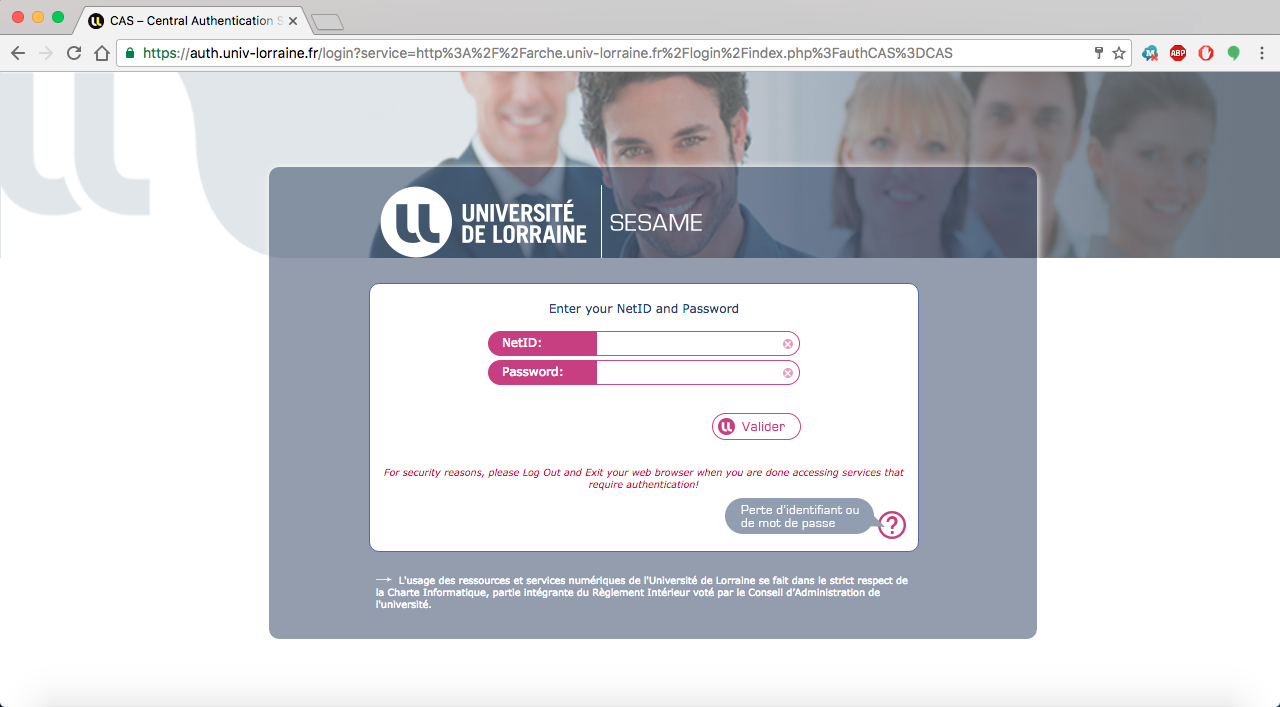
\includegraphics[scale=0.4]{image/CAS.png}}
\end{center}
\vspace{3cm}
\begin{flushleft}
\hspace{1cm}Une fois la connexion établie, l'étudiant peut télécharger les documents dont il a besoin pour son stage avec en vert, les éléments qu'il peut télécharger, et en rouge, ceux qu'il ne peut pas.
\end{flushleft}
\begin{center}
\centerline{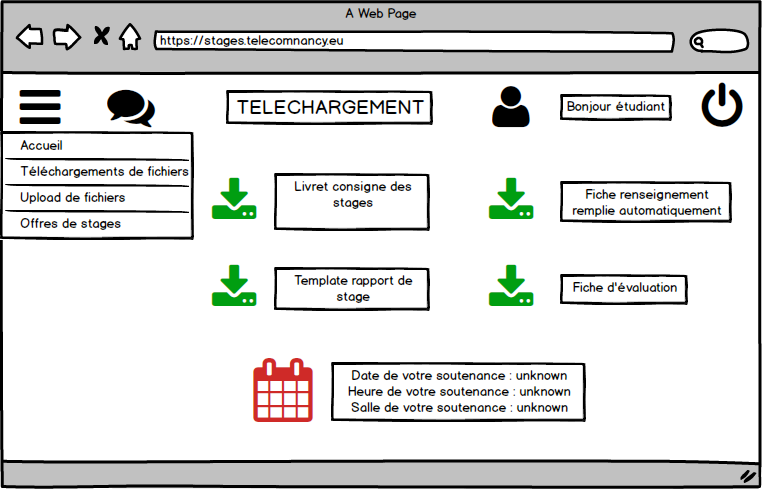
\includegraphics[scale=0.65]{image/DownloadEleve.png}}
\end{center}
\vspace{8cm}
\begin{flushleft}
\hspace{1cm}Il peut aussi trouver les fichiers ou données qu'il doit envoyer sur la plateforme. Avec un vert les fichiers qu'il à déjà envoyés et en rouge, les fichiers non envoyés.
\end{flushleft}
\begin{center}
\centerline{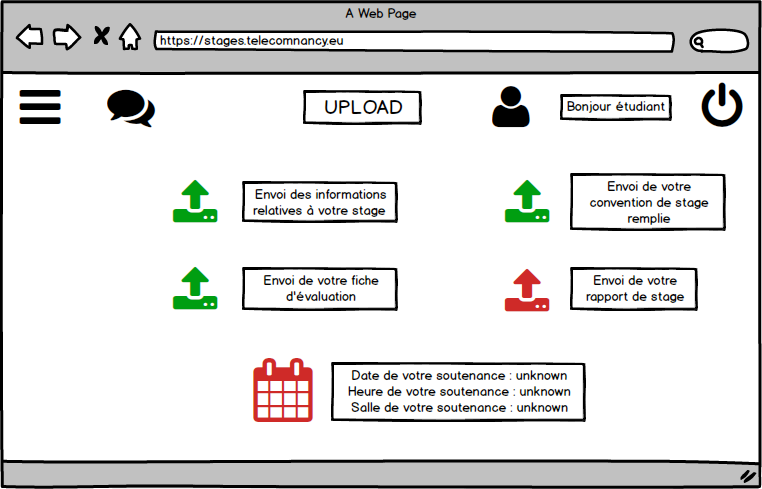
\includegraphics[scale=0.65]{image/uploadeleve.png}}
\end{center}
\begin{flushleft}
\vspace{8cm}
\hspace{1cm}Pour ce qui concerne l'envoi des informations relatives au stage, l'élève doit envoyer un certain nombre d'informations nécessaires à la génération automatique de la fiche.
\end{flushleft}
\begin{center}
\centerline{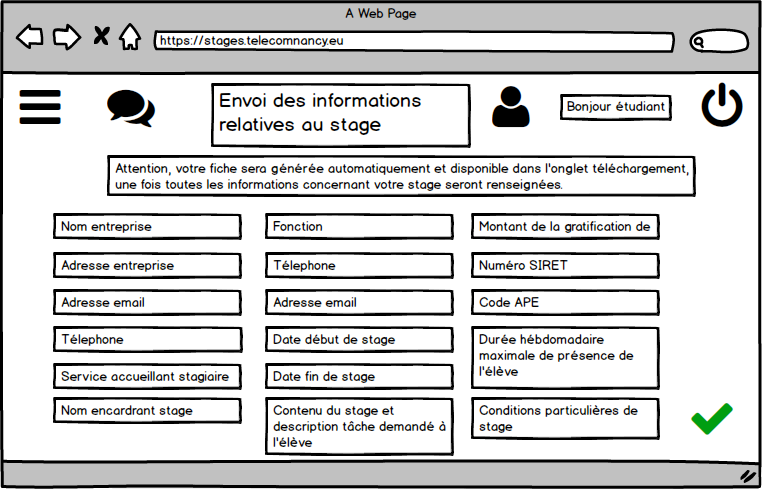
\includegraphics[scale=0.65]{image/inforelativesstages.png}}
\end{center}

\section{Besoins fonctionnels}

Voici les besoins fonctionnels liés aux \textbf{Étudiants} :
\begin{center}
\vspace {0.5cm}
\begin{tabular}{|p{5cm}|p{7cm}|p{2cm}|}
  \hline
  \textbf {Fonction} & \textbf {Description} & \textbf {Priorité} \\
  \hline
  En tant qu'étudiant, je dois m'authentifier avec mes identifiants UL pour accéder à mon espace. & L'authentification UL via le CAS est nécessaire pour accéder aux fonctionnalités de l'application. & Haute\\
  \hline
  En tant qu'étudiant, je peux déposer mon rapport de stage. & Le dépôt du rapport doit être effectué avant une date buttoir. & Haute\\ 
  \hline
  En tant qu'étudiant, je peux saisir les informations relatives au stage composant la convention et la fiche de renseignements. & L'application permet l’édition en ligne de la convention de stage et de la fiche de renseignements propre à l'étudiant. & Moyenne\\
  \hline
  En tant qu'étudiant, je peux consulter les dates de soutenance qui me sont affectées. & L'application conserve et met à disposition toutes les dates de soutenances liées à l'étudiant & Moyenne\\
  \hline
  En tant qu'étudiant, je peux échanger avec mon encadrant de stage des informations concernant le stage. & L'application permet d'échanger des mails via le protocole STMP. & Basse\\
  \hline
  En tant qu'étudiant, je peux accéder à des offres de stages. & Ces offres seront listées dans un PDF. & Basse\\
  \hline
  En tant qu'étudiant, je peux accéder au livret de l'élève. & L'application conserve et met à disposition la dernière version du livret de l'élève. & Basse\\
  \hline
  En tant qu'étudiant, je peux télécharger la fiche d'évaluation, et la déposer une fois remplie. & L'application conserve et met à disposition la fiche d'évaluation. Le dépôt de cette dernière doit être effectué avant une date buttoir. & Basse\\
  \hline  
  En tant qu'étudiant, je peux accéder au template de mémoire d'ingénieur. & L'application conserve et met à disposition un template de mémoire d'ingénieur. & Basse\\
  \hline
\end{tabular}
\end{center}
\vspace{1cm}
Voici les besoins fonctionnels liés au \textbf{Service informatique} :
\begin{center}
\begin{tabular}{|p{5cm}|p{7cm}|p{2cm}|}
  \hline
  \textbf {Fonction} & \textbf {Description} & \textbf {Priorité} \\
  \hline
  En tant que membre du service informatique de l'école, je peux accéder et modifier tous les paramètres de l'application. & Le membre du service informatique peut accéder au code source de l'application et à son hébergeur pour d'éventuelles maintenances.  & Haute\\
  \hline
  En tant que membre du service informatique de l'école, je peux répondre aux requêtes (d'aide ou autres) des autres utilisateurs. & Les utilisateurs peuvent échanger des mails grâce au protocole STMP fourni par l'application. & Basse\\ 
  \hline
\end{tabular}
\end{center}

\vspace{1cm}
Voici les besoins fonctionnels liés à la \textbf{Secrétaire des stages} :
\begin{center}
\begin{tabular}{|p{5cm}|p{7cm}|p{2cm}|}
  \hline
  \textbf {Fonction} & \textbf {Description} & \textbf {Priorité} \\
  \hline
  En tant que secrétaire des stages, je peux mettre en ligne des fichiers dont les élèves ont besoin pour leur stage, pour chaque année. & L'application permet le dépôt de fichiers nécessaires aux élèves dans différentes sections de l'application. & Haute\\
  \hline
  En tant que secrétaire des stages, je peux accéder aux données mises en ligne par les élèves. & L'application conserve et met à disposition de la secrétaire des stages tous les fichiers et données mis en ligne par les élèves. & Haute\\ 
  \hline
  En tant que secrétaire des stages, je peux modifier le statut des élèves. & L'application permet à la secrétaire des stages d'administrer l'année d'appartenance de chaque élève. & Haute\\ 
  \hline
\end{tabular}
\end{center}

\vspace{1cm}
Voici les besoins fonctionnels liés aux \textbf{Professeurs} :
\begin{center}
\begin{tabular}{|p{5cm}|p{7cm}|p{2cm}|}
  \hline
  \textbf {Fonction} & \textbf {Description} & \textbf {Priorité} \\
  \hline
  En tant que professeur, je peux avoir accès à toutes les informations concernant les stages des élèves. & L'application fournit aux professeurs toutes les informations relatives aux stages des élèves. & Haute\\
  \hline
  En tant que professeur responsable de stages, je peux valider ou non un stage. & L'application permet aux professeurs responsable de stages de valider ou non en ligne les stages qui leur ont été confiés. & Moyenne\\ 
  \hline
  En tant que professeur, je peux contacter les élèves dont je corrige leur rapport de stage. & Les professeurs peuvent échanger des mails avec les élèves concernés via le protocole STMP. & Basse\\ 
  \hline
\end{tabular}
\end{center}

\vspace{1cm}
Voici les besoins fonctionnels liés au \textbf{Directeur} :
\begin{center}
\begin{tabular}{|p{5cm}|p{7cm}|p{2cm}|}
  \hline
  \textbf {Fonction} & \textbf {Description} & \textbf {Priorité} \\
  \hline
  En tant que directeur, je peux avoir accès à toute l'application sans restriction de droit. & L'application considère le directeur comme un administrateur et lui confère tous les droits. & Haute\\
  \hline
  En tant que directeur, je peux valider ou non les stages 3A. & L'application permet au directeur de valider ou non en ligne les stages de 3A & Haute\\ 
  \hline
  En tant que directeur, je peux contacter les élèves dont je corrige leur rapport de stage. & Le directeur peut échanger des mails avec les élèves concernés via le protocole STMP. & Basse\\ 
  \hline
\end{tabular}
\end{center}

\vspace{1cm}
Voici les besoins fonctionnels qui ne sont pas liés au utilisateurs :
\begin{center}
\begin{tabular}{|p{5cm}|p{7cm}|p{2cm}|}
  \hline
  \textbf {Fonction} & \textbf {Description} & \textbf {Priorité} \\
  \hline
  L'application vérifie chaque fichier mis en ligne. & Un antivirus intégré vérifiera chaque fichier déposé par les utilisateurs et transmettra un rapport au service informatique dans le cas d'un problème de sécurité ou d'une tentative de piratage. & Haute\\
  \hline
\end{tabular}
\end{center}


\section{Besoins comportementaux}

\subsection{Diagrammes de séquence des cas d'utilisation}
%AUTENTIFICATION :
\begin{center}
	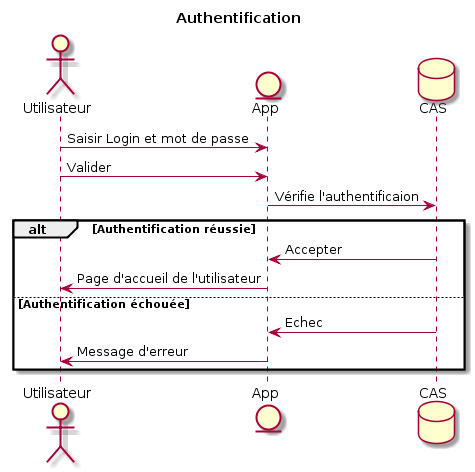
\includegraphics[scale=0.55]{image/authentification.png}
\end{center}
%\begin{center}
%	\textbf{Figure 3.3.1.} S'autentifier
%\end{center}
\hspace{1cm}Les utilisateurs de l'application doivent s'y authentifier à son ouverture. Ils utilisent pour cela leurs identifiants de l'Université de Lorraine.

%ACCES AU LIVRET DE L'ELEVE :
\begin{center}
	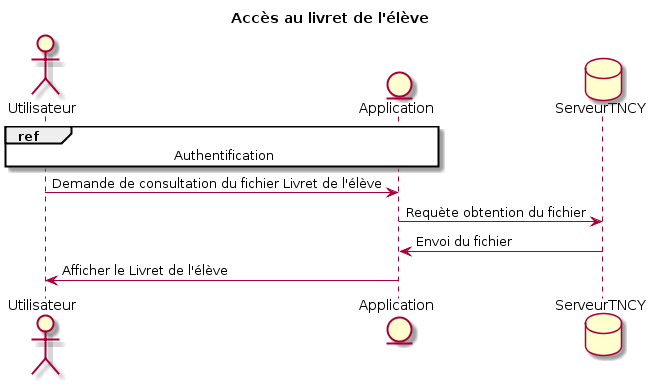
\includegraphics[scale=0.55]{image/accesLivretEleve.png}
\end{center}
\hspace{1cm}Les étudiants doivent pouvoir télécharger le livret de l'élève depuis l'application ; pour ce faire, ils doivent d'abord se connecter au service.

%SAISIE DES INFORMATIONS RELATIVES AU STAGE :
\begin{center}
	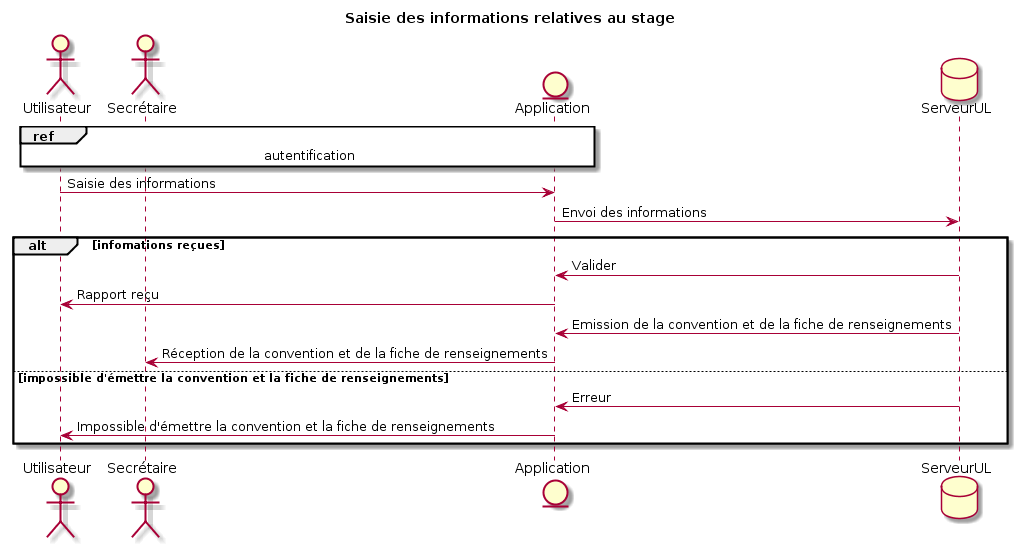
\includegraphics[scale=0.4]{image/saisieInfosStage.png}
\end{center}
\hspace{1cm}Plutôt que de remplir la fiche d'informations relatives au stage et la convention qui doivent ensuite être recopiées manuellement par le secrétarie des stages, l'étudiant a la possibilité d'entrer directement ces informations dans l'application qui émet ensuite automatiquement la convention à signer.

%DEPOSE DU RAPPORT :
\begin{center}
	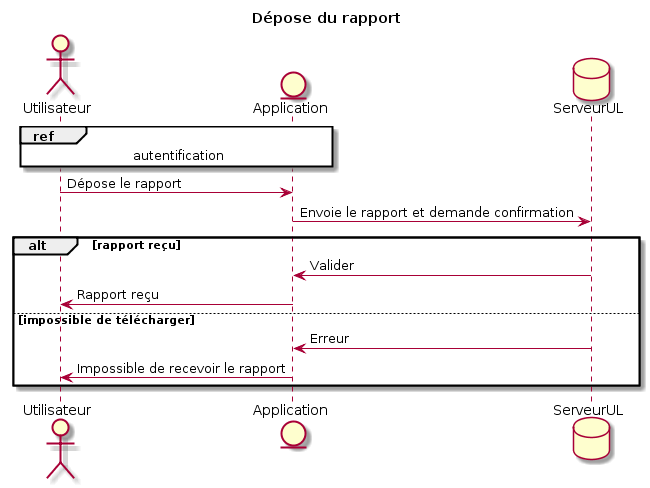
\includegraphics[scale=0.55]{image/deposeRapport.png}
\end{center}
\hspace{1cm}L'une des fonctionnalités principales de l'application est de permettre à l'étudiant de déposer son rapport de stage pour que celui-ci soit corrigé. L'application lui indique si la réception du document a eu lieu ou pas.

%OBTENTION DES DATES DE SOUTENANCE :
\begin{center}
	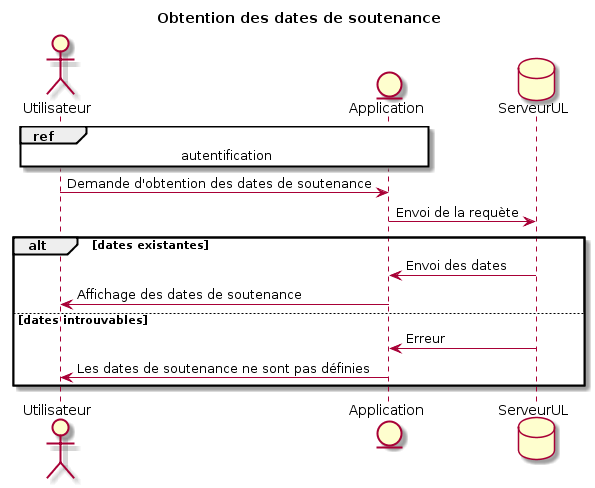
\includegraphics[scale=0.55]{image/obtentionDatesSoutenance.png}
\end{center}
\hspace{1cm}Les étudiants peuvent obtenir les dates de soutenance qui leur sont affectées par l'intermédiaire de l'application après authentification.

%TELECHARGEMENT DE LA FICHE D'EVALUATION :
\begin{center}
	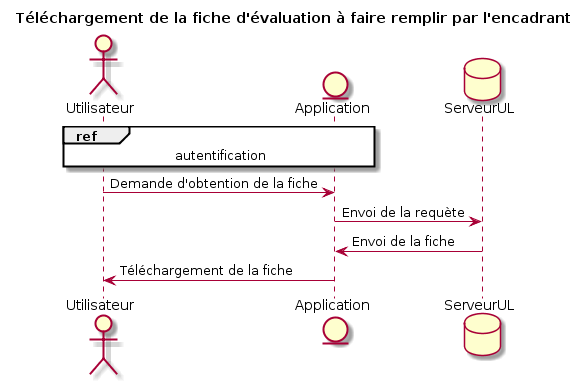
\includegraphics[scale=0.55]{image/telechargementFicheEvaluation.png}
	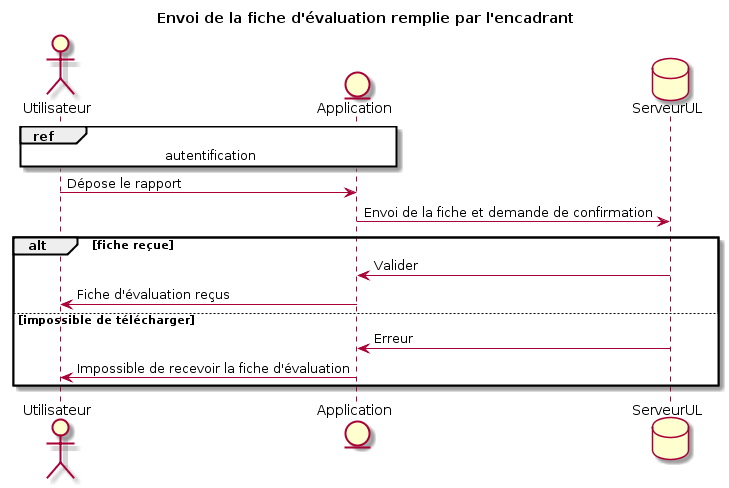
\includegraphics[scale=0.55]{image/envoiFicheEvaluation.png}
\end{center}
\hspace{1cm}L'application permet aux étudiant de télécharger la fiche d'évaluation par le maître de stage pour la lui faire remplir. Après cette opération, ils ont la possibilité de déposer la fiche remplie sur la plateforme.

%MISE EN LIGNE DE DOCUMENTS PAR LE SECRETARIAT DES STAGES :
\begin{center}
	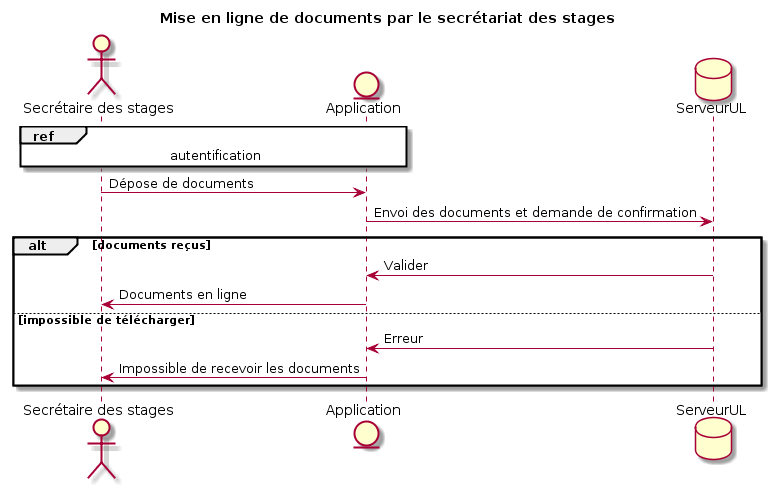
\includegraphics[scale=0.55]{image/miseEnLigneDocumentsParSecretaire.png}
\end{center}
\hspace{1cm}Pour que les étudiants puissent télécharger les documents dont ils ont besoin pour le bon déroulement de leur stage, le secrétariat des stages doit pouvoir les mettre en ligne, accessibles par le biais de l'application développée ici.

%ACCES AUX DONNEES MISES EN LIGNE PAR LES ETUDIANTS PAR LE SECRETARIAT DES STAGES :
\begin{center}
	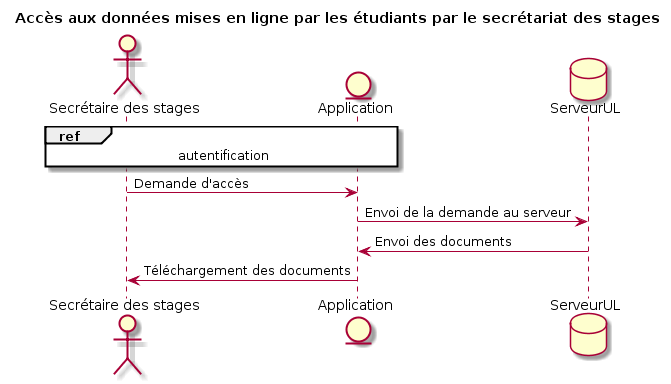
\includegraphics[scale=0.55]{image/accesDonneesParSecretaire.png}
\end{center}
\hspace{1cm}Après que les étudiants ont entré les informations relatives au stage dans l'application, le secrétariat des stages y a accès ainsi qu'a la convention générée automatiquement.

%MODIFICATION DE L'ANNEE D'APPARTENANCE D'UN ETUDIANT PAR LE SECRETARIAT DES STAGES :
\begin{center}
	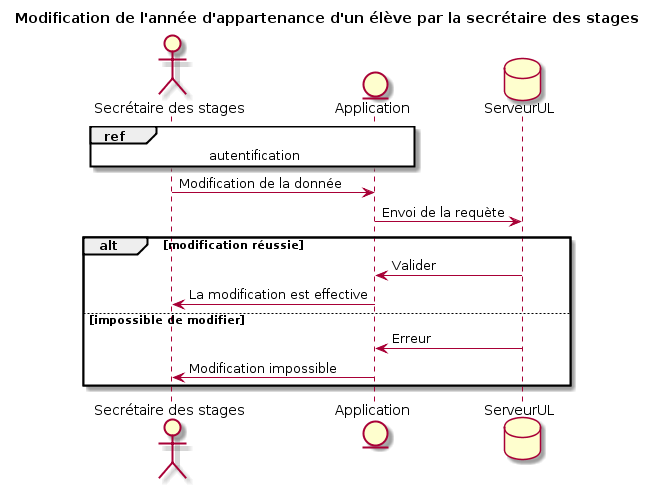
\includegraphics[scale=0.55]{image/modifAnneeParSecretaire.png}
\end{center}
\hspace{1cm}Le secrétariat des stages a la charge de modifier l'année d'appartenance d'un étudiant lorsque son stage est validé par le professeur référent.

%ACCES AUX DONNEES MISES EN LIGNE PAR LES ETUDIANTS PAR LE PROFESSEUR RESPONSABLE :
\begin{center}
	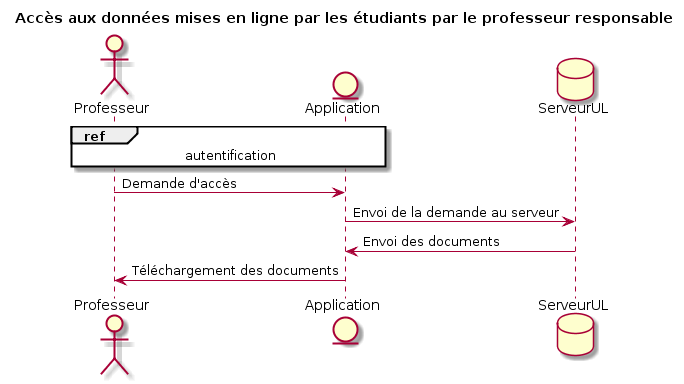
\includegraphics[scale=0.55]{image/accesDonneesParProfesseur.png}
\end{center}
\hspace{1cm}Comme pour le secrétariat des stages, après que les étudiants ont entré les informations relatives au stage dans l'application, leur professeur répérent y a accès.

%VALIDATION OU NON DU STAGE PAR LE PROFESSEUR :
\begin{center}
	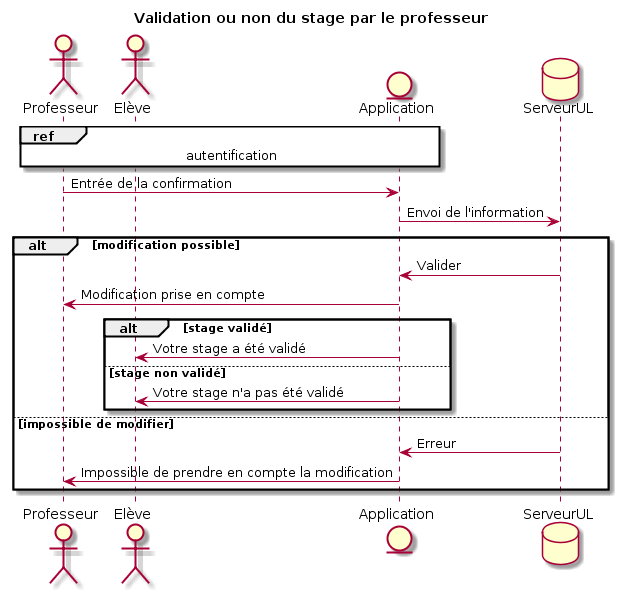
\includegraphics[scale=0.55]{image/validationStage.png}
\end{center}
\hspace{1cm}Après qu'il a corrigé le rapport de stage de l'étudiant et qu'il a consulté la fiche d'évaluation du stage par l'encadrant, le professeur référent a la possibilité de valider ou non le stage de l'élève.

\subsection{Diagrammes de cas d'utilisation}
%DIAGRAMME DE CAS D'UTILISATION DE L'ETUDIANT :
\subsubsection{Diagrammes de cas d'utilisation de l'étudiant}
\begin{center}
	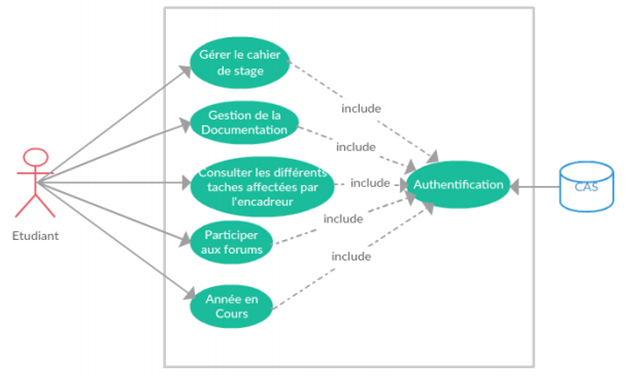
\includegraphics[scale=0.55]{image/casutilisationetudiant.png}
\end{center}
%DESCRIPTION DE CAS D'UTILISATION ANNEE EN COURS :
\subsubsection{Description de cas d'utilisation de l'année en cours}
\begin{center}
	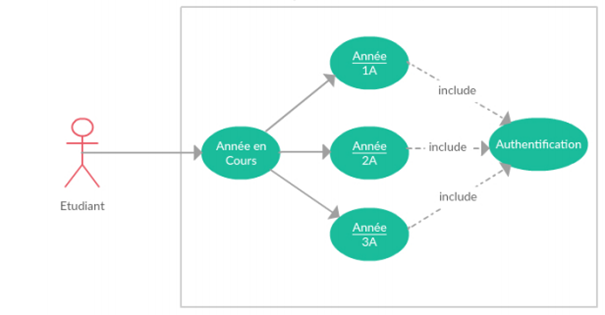
\includegraphics[scale=0.55]{image/descriptiondecasanneencours.png}
\end{center}
%DIAGRAMME DE CAS D'UTILISATION DE L'ENCADREUR :
\subsubsection{Diagrammes de cas d'utilisation de l'encadreur}
\begin{center}
	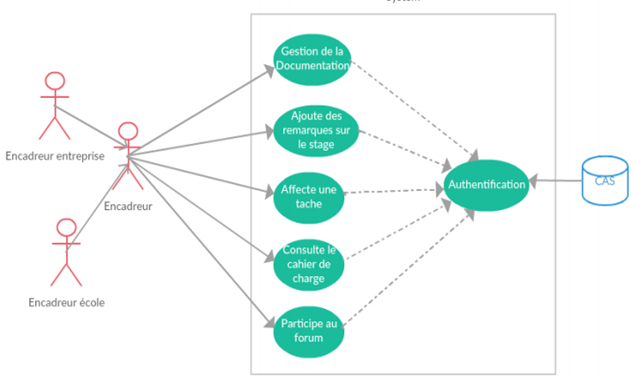
\includegraphics[scale=0.55]{image/casutilisationencadreur.png}
\end{center}
%DIAGRAMME DE CAS D'UTILISATION DU DIRECTEUR :
\subsubsection{Diagrammes de cas d'utilisation du directeur}
\begin{center}
	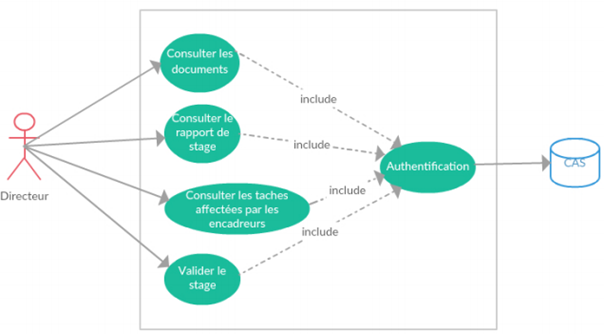
\includegraphics[scale=0.55]{image/casutilisationdudirecteur.png}
\end{center}
%DIAGRAMME DE CAS D'UTILISATION DE L'ADMINISTRATEUR :
\subsubsection{Diagrammes de cas d'utilisation de l'administrateur}
\begin{center}
	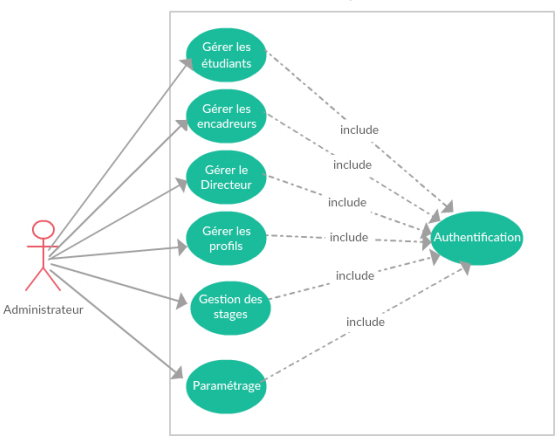
\includegraphics[scale=0.55]{image/casutilisationdeadministrateur.png}
\end{center}


\chapter{AUTRES BESOINS NON FONCTIONNELS}

\section{Besoins liés à la performance}
\hspace{1cm}L'application doit pouvoir fonctionner sur des smartphones et des tablettes et est de ce fait limitée au niveau de son utilisation de mémoire vive (qui ne doit pas être supérieure à 500Mo). Elle doit aussi pouvoir charger rapidement : avec une connexion internet classique, les pages internet ne doivent pas prendre plus de 10 secondes pour charger.\\

\hspace{0.6cm}Pendant la période précédant les stages où les élèves doivent pouvoir entrer les informations sur leurs stages, le site ne doit pas rester hors ligne plus d'une heure en cas de problème technique avec le serveur. Au moment du rendu des rapports de stages et pour que les étudiants ne soient pas pénalisés par un facteur qu'ils ne maîtrisent pas, le site ne doit pas rester hors-ligne plus de quelques minutes. Par ailleurs, il doit aussi, à cette période, supporter jusqu'à 200 connexions sumultanées.

\subsection{Besoins liés à la sécurité}
\hspace{1cm}Les informations d'un étudiant doivent être privées et accessibles uniquement par celui-ci et la scolarité. Parallèlement, le rapport de stage d'un étudiant ne doit être visible que par le professeur reponsable qui est chargé de sa correction et la scolarité. Cela est implémentable grâce au passage par le CAS de l'UL (c'est-à-dire l'authentification des utilisateurs).\\

\hspace{0.6cm}Il est par ailleurs souhaitable que les données manipuler par l'application soient chiffrées pour éviter tout problème d'obtention apr une personne non-autorisée.

\subsection{Besoins liés à la qualité du produit }
\hspace{1cm}L'application doit être implémentée de façon à être facilement utilisable et intuitive. L'esthétisme doit aussi être un point important, et l'application doit s'adapter au support de l'utilisateur sans que l'interface devienne inutilisable.\\

\hspace{0.6cm}L'application permet aux utilisateurs d'être aidé par le service informatique en cas et problème et d'avoir accès à un manuel utilisateur décrivant les différentes fonctionnalités de l'application et leur utilisation.





\chapter{AUTRES BESOINS}



\appendix
\chapter*{ANNEXE A : Dictionnaire de données}
\addcontentsline{toc}{chapter}{ANNEXE A : Dictionnaire de données}

\begin{center}
	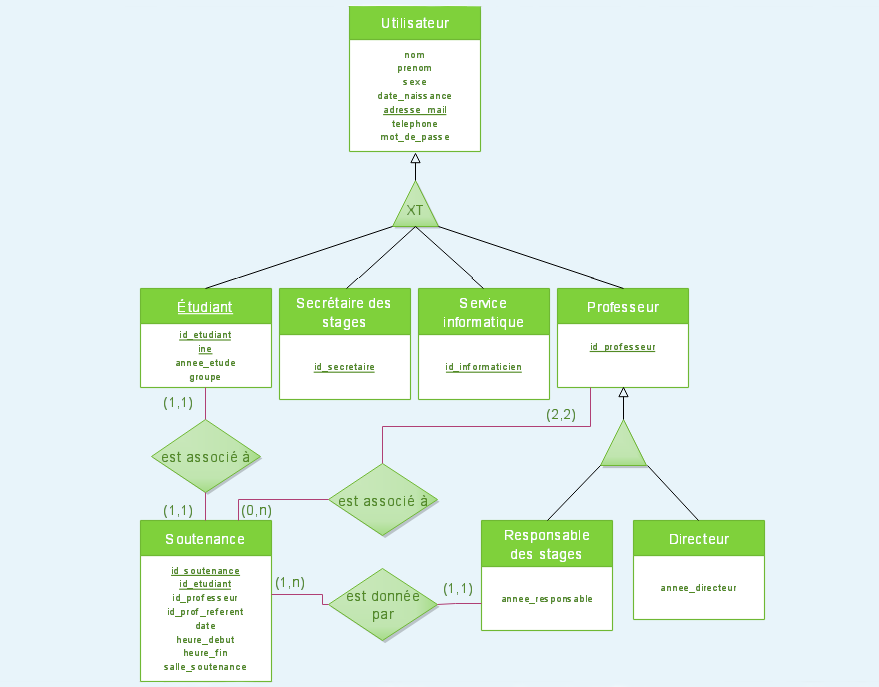
\includegraphics[scale=0.45]{image/diagentiassoc.png}
	\vspace {0.5cm}
	\textbf{Figure 5.1.1.} Diagramme entités-associations
\end{center}

\vspace {4cm}
\begin{center}
\textbf 
{Étudiant}
\vspace {0,5cm}

\begin{tabular}{|c|c|c|c|}
  \hline
  \textbf {Champ} & \textbf {Type} & \textbf {Description} & \textbf {Commentaires} \\
  \hline
  id_etudiant & varchar2 & identifiant de l'étudiant UL & clé primaire\\
  \hline
  nom & varchar2 & nom de l'élève &  \\
  \hline
  prénom & varchar2 & prénom(s) de l'étudiant &  \\
  \hline
  sexe & varchar2 & sexe de l'étudiant &  \\
  \hline
  date_naissance & date & date de naissance de l'étudiant &  \\
  \hline
  ine & int & numéro INE de l'étudiant & clé primaire \\
  \hline
  annee_etude & varchar2 & l'année en cours de l'élève (1A, 2A, 3A) &  \\
  \hline
  adresse_mail & varchar2 & adresse mail de l'étudiant & clé primaire\\
  \hline
  telephone & varchar2 & numéro de téléphone de l'étudiant &  \\
  \hline
  groupe & int & groupe de l'étudiant &  \\
  \hline
  mot_de_passe & varchar2 & mot de passe de l'étudiant &  \\
  \hline
\end{tabular}

\vspace {1cm}
\textbf 
{Soutenance}
\vspace {0,5cm}

\begin{tabular}{|c|c|c|c|}
  \hline
  \textbf {Champ} & \textbf {Type} & \textbf {Description} & \textbf {Commentaires} \\
  \hline
  id_soutenance & int & id de la soutenance & clé primaire\\
  \hline
  id_etudiant & varchar2 & identifiant de l'étudiant UL & clé primaire\\
  \hline
  id_professeur & varchar2 & id du professeur assistant à la soutenance &  \\
  \hline
  id_professeur_referent & varchar2 & identifiant du professeur référent &  \\
  \hline
  date & date & date de soutenance &  \\
  \hline
  heure_debut & time & heure de début de soutenance &  \\
  \hline
  heure_fin & time & heure de fin de soutenance &  \\
  \hline
  salle_soutenance & varchar2 & salle accueillant la soutenance &  \\
  \hline
\end{tabular}

\vspace {1cm}
\textbf 
{Service Informatique}
\vspace {0,5cm}

\begin{tabular}{|c|c|c|c|}
  \hline
  \textbf {Champ} & \textbf {Type} & \textbf {Description} & \textbf {Commentaires} \\
  \hline
  id_informaticien & varchar2 & identifiant de l'informaticien UL & clé primaire\\
  \hline
  nom & varchar2 & nom de l'informaticien & \\
  \hline
  prenom & varchar2 & prénom(s) de l'informaticien &  \\
  \hline
  sexe & varchar2 & sexe de l'informaticien &  \\
  \hline
  adresse_mail & varchar2 & adresse mail de l'informaticien & clé primaire  \\
  \hline
  mot_de_passe & varchar2 & mot de passe de l'informaticien &  \\
  \hline
  telephone & varchar2 & numéro de téléphone du service informatique &  \\
  \hline
\end{tabular}

\vspace {2cm}
\textbf 
{Directeur}
\vspace {0,5cm}

\begin{tabular}{|c|c|c|c|}
  \hline
  \textbf {Champ} & \textbf {Type} & \textbf {Description} & \textbf {Commentaires} \\
  \hline
  id_directeur & varchar2 & identifiant du directeur UL & clé primaire\\
  \hline
  nom & varchar2 & nom du directeur & \\
  \hline
  prenom & varchar2 & prénom(s) du directeur &  \\
  \hline
  sexe & varchar2 & sexe du directeur &  \\
  \hline
  adresse_mail & varchar2 & adresse mail du directeur & clé primaire  \\
  \hline
  mot_de_passe & varchar2 & mot de passe du directeur &  \\
  \hline
  telephone & varchar2 & numéro de téléphone du directeur &  \\
  \hline
\end{tabular}

\vspace {1cm}
\textbf 
{Secrétaire des stages}
\vspace {0,5cm}

\begin{tabular}{|c|c|c|c|}
  \hline
  \textbf {Champ} & \textbf {Type} & \textbf {Description} & \textbf {Commentaires} \\
  \hline
  id_secretaire & varchar2 & identifiant de la secrétaire UL & clé primaire\\
  \hline
  nom & varchar2 & nom de la secrétaire & \\
  \hline
  prenom & varchar2 & prénom(s) de la secrétaire &  \\
  \hline
  sexe & varchar2 & sexe de la secrétaire &  \\
  \hline
  date_naissance & date & date de naissance de la secrétaire &  \\
  \hline
  adresse_mail & varchar2 & adresse mail de la secrétaire & clé primaire  \\
  \hline
  mot_de_passe & varchar2 & mot de passe de la secrétaire &  \\
  \hline
  telephone & varchar2 & numéro de téléphone de la secrétaire &  \\
  \hline
\end{tabular}

\vspace {1cm}
\textbf 
{Responsable des stages}
\vspace {0,5cm}

\begin{tabular}{|c|c|c|c|}
  \hline
  \textbf {Champ} & \textbf {Type} & \textbf {Description} & \textbf {Commentaires} \\
  \hline
  id_responsable & varchar2 & identifiant du responsable des stage UL & clé primaire\\
  \hline
  nom & varchar2 & nom du responsable des stages & \\
  \hline
  prenom & varchar2 & prénom(s) du responsable des stages &  \\
  \hline
  sexe & varchar2 & sexe du responsable des stages &  \\
  \hline
  date_naissance & date & date de naissance du responsable des stages &  \\
  \hline
  annee_responsable & varchar2 & responsable des stages de l'année (1A,2A,3A) &  \\
  \hline
  adresse_mail & varchar2 & adresse mail du responsable des stages & clé primaire  \\
  \hline
  mot_de_passe & varchar2 & mot de passe du responsable des stages &  \\
  \hline
  telephone & varchar2 & numéro de téléphone du responsable des stages &  \\
  \hline
\end{tabular}

\vspace {3cm}
\textbf 
{Professeur}
\vspace {0,5cm}

\begin{tabular}{|c|c|c|c|}
  \hline
  \textbf {Champ} & \textbf {Type} & \textbf {Description} & \textbf {Commentaires} \\
  \hline
  id_professeur & varchar2 & identifiant du professeur UL & clé primaire\\
  \hline
  nom & varchar2 & nom du professeur & \\
  \hline
  prenom & varchar2 & prénom(s) du professeur &  \\
  \hline
  sexe & varchar2 & sexe du professeur &  \\
  \hline
  date_naissance & date & date de naissance du professeur &  \\
  \hline
  adresse_mail & varchar2 & adresse mail du professeur & clé primaire  \\
  \hline
  mot_de_passe & varchar2 & mot de passe du professeur &  \\
  \hline
  telephone & varchar2 & numéro de téléphone du professeur &  \\
  \hline
\end{tabular}

\end{center}

\end{document}
